\chapter{Conclusions and discussion} \label{chap_conclusions}

This thesis culminates a multifaceted exploration into the convergence of \gls{ca} with
\gls{ns}. We have drawn upon the author's firsthand experience in designing Software
Architectures used rigorous theoretical research and created a practical and working
Software Artifact. The primary objective was to investigate the convergence between \gls{ca}
and \gls{ns}, by analyzing their principles and design elements through theory and
practice. This Chapter will summarize the findings into a research conclusion.

\section{Conclusion}

A noteworthy distinction between \gls{ns} and \gls{ca} lies in their foundational roots.
\gls{ns} is a product of computer science research built upon formal theories and
principles derived from rigorous scientific investigation. Although, throughout this
thesis, \gls{ns} is referred to as a development approach, it is a part of Computer
Science.

Stability and evolvability are concepts not directly referenced in the literature of
\gls{ca}, but very much converges with the goal of \textcite[31]{mannaert_normalized_2016}.
Clearly depicted in Table \ref{tab_convergence_principles_summarized} The attentive reader
surely observes the shared emphasis on modularity and the separation of concerns, as all
SOLID principles have a stong convergence with \gls{soc}. Both approaches attempt to
achieve low coupling and high cohesion. In addition, \gls{ca} add the dimensions of
dependency management as usefull measure to improve maintainability and manage modularity.

The Transparency of Data versions appears to be underrepresented in the SOLID principles
of \gls{ca}. \gls{dvt} is primarily supported by the \gls{srp} of \gls{ca}, as evidenced
by the presence of ViewModels, RequestModels, ResponseModels, and Entities in the
Artifact. It is worth noting that these are an integral part of the design elements of
\gls{ca}. While \gls{ca} does address \gls{dvt} through the \gls{srp}, a more
comprehensive representation and integration of \gls{dvt} as a principle within the
principles of \gls{ca} will improve the convergence of \gls{ca} with \gls{ns}, potentially
improving the stability and evolvability of Software Systems based on \gls{ca}.

As indicated in Table \ref{tab_convergence_elements_summarized}, seems to lack a strong
foundation for receiving external triggers in it's desing phylosophy. This is partially
represented by the Controller element, however this element tends to be use for web
enabled environments like websites and Restful APIs. This may result in a less
comprehensive approach to receiving external triggers across various technologies or
systems.

A critical difference between \gls{ca} and \gls{ns} lies in their approach to handling
state. \gls{ca} does not explicitly address state management in its principles or design
elements. At the same time, \gls{ns} provides the principle of Separation of State,
ensuring that state changes within a Software System are stable and evolvable. This
principle can be crucial in developing scalable and high-performance systems, as it
isolates state changes from the rest of the system, reducing the impact of state-related
dependencies and side effects. 

The findings can only leads to the conclusion that the convergence between \gls{ca} and
\gls{ns} is incomplete because \gls{ca} needs specific state management principles. As a
result, \gls{ca} cannot fully ensure stable and evolvable software artifacts as defined by
\gls{ns}.


\section{Discussion}

In this research, the convergence between \gls{ca} and \gls{ns} has been thoroughly
investigated. While it has been demonstrated that the convergence between these two
approaches is not complete, the combination of both methodologies is highly beneficial for
a variety of reasons. The primary advantage of this convergence lies in the complementary
nature of \gls{ca} with \gls{ns}, where each approach provides strengths that can be
leveraged to address a strong architectural design. 

Clean Architecture offers a well-defined, practical, and modular structure for software
development. Its principles, such as SOLID, guide developers in creating maintainable,
testable, and scalable systems. This architectural design approach is highly suitable for
a wide range of applications and can be easily integrated with the theoretical foundations
provided by \gls{ns}. Conversely, the NS approach offers a more comprehensive theoretical
underpinning for evolvable systems, guiding achieving stability and evolvability.

Furthermore, the popularity and widespread adoption of Clean Architecture in the software
development community can be advantageous for Normalized Systems. As more developers
become familiar with CA and recognize its value to software design, incorporating \gls{ns}
principles becomes more accessible, leading to increased adoption and improved software
systems.

\section{Limitations}

In this research, the artifacts created to demonstrate the convergence between \gls{ca}
and \gls{ns} have shown promising results. However, it is essential to recognize these
artifacts' limitations, particularly in implementing \gls{ns} principles such as the
Separation of State Principle and the Trigger Element. These limitations must be
acknowledged to guide future work and refinement of the combined architectural design
approaches.

One of the primary limitations of the artifacts lies in their incomplete representation of
the Separation of State principle. This principle is crucial in \gls{ns} to ensure proper
handling of state changes while achieving stability and evolvability. While the artifacts
incorporate some aspects of state management, they fall short of fully implementing the
Separation of State principle as \gls{ns} prescribes. 

The other limitation of the artifacts is their lack of a comprehensive Trigger Element, an
essential element of \gls{ns}. The Trigger Element manages external triggers while
ensuring that software remains stable and evolvable. In the artifacts, incorporating the
Trigger Element is limited, primarily relying on the Controller element from \gls{ca}.
While this approach may be sufficient for web-enabled environments such as websites and
RESTful APIs, it may not be adequate for a broader range of requirements.
\section{Reflections} \label{chap_reflection}

This section will dive into my enriching experiences and invaluable learnings acquired
while working on this research and thesis and is inspired by one of the master classes
about the \gls{ee} discipline. \gls{ee} encourages using grounded methodologies and
theories, like Five Way Framework, to comprehend the inner workings of an enterprise
\parencite[262]{dietz_enterprise_2020}. I will apply the so-called Five Way Framework to
reflect on this research. By incorporating the Five Way Framework into the section, I
aspire to coherently showcase my learnings and reflections, shedding light on my thought
processes, strategies, modeling techniques, working methodologies, and support mechanisms.

\begin{figure}[H]
    \centering
    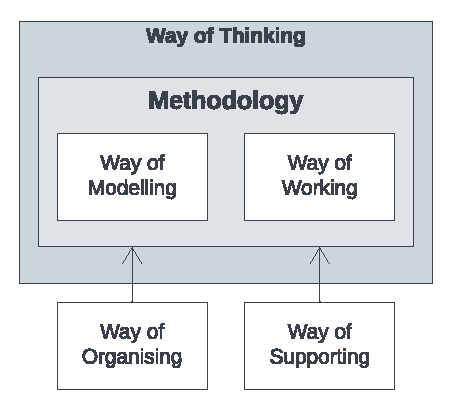
\includegraphics[width=0.5\textwidth]{figures/5ways.pdf}
    \caption[The Five Way Framework]{The Five Way Framework, inspired by \textcite{dietz_enterprise_2020}}
    \label{fig_5ways}
\end{figure}

\subsection{Way of Thinking}

Early in my career, I became obsessed with Software Quality and Maintainability. The
\gls{ns} theory shifted the obsession toward Stability and Evolvability. Gaining a
thorough understanding of the essential principles of this theory has boosted my
confidence in making informed decisions regarding all aspects of architecture, not just
limited to software.

As a Domain Architect, my job involved creating software products using the \gls{mdd}
paradigm. Initially, I was skeptical about this approach based on my early experiences.
The theory of \gls{ns} taught me to understand better the reasoning and characteristics of
code generation, on which I then realized that my skepticism was more about the process
caused as an effect on the implementation of the \gls{mdd}. The knowledge of \gls{ns}
helped me gain a clearer vision and helped me push the roadmap on the \gls{mdd} framework
in the right direction.

\subsection{Way of Modeling}

To explain the implementation concepts of the artifact, I looked into various modeling
languages. Archimate was the first option I considered. However, during one of the \gls{ee}
masterclasses, I learned the hard way that Archimate is not always the best choice for
communicating your models to a broad audience. I thought about using basic "boxes and
arrows" but decided to use the UML2 standard because it is a formal modeling language.

\subsection{Way of Working}

I very much enjoyed designing and creating the C\# artifacts. In hindsight, I enjoyed it
so much that I put in way too much effort than was needed. I was very curious about the
aspects of code generation, the effect of code generation on stable and evolvable
artifacts, and meta-circularity characteristics. I am confident I could have arrived at
the same conclusions presented in this thesis using a manually built Restful C\# artifact.
However, the insights I gained on the subjects of code expansion are of invaluable value
to me. Therefore, I am very pleased and satisfied that I took the effort to build the Code
Expander as a primary artifact. 

The \gls{ns} theorems are formulated very clearly and abstractly, making them also
applicable outside the software engineering field. During the masterclasses, we learned
about the application of \gls{ns} in the domains of Firewalls, Document management
systems, and Evolvable Business Processes. I also experienced benefits in structuring and
maintaining my Thesis document using \gls{vscode} and Latex by applying the principle of
\gls{soc} in managing the various chapters and sections. 

\subsection{Way of Organizing}

I should have been able to finish sooner. I was one of the first with a research topic and
started working on my artifact in the first month when starting this journey. The artifact
was as good as ready before the summer holidays of the first year. Unfortunately, I
postponed writing the thesis until a later moment. I want to think that next time I will
start sooner, but knowing myself, I need some pressure to perform the less fun tasks, like
writing this thesis.

The review process seemed difficult and sometimes even problematic for a couple of
reasons. Next time I will ensure having the proper tools and agree on procedures to
improve reviews from multiple proofreaders. Secondly, I noticed that having multiple
proofreaders sometimes steers in opposite directions. This sometimes affected my ability
to make decisions and negatively affected my confidence. Having a joined review document,
where all proofreaders can leave comments, will significantly improve this experience for
me and my proofreaders. Then there is the personal aspect of sometimes taking things too
personally, grounded in a lack of self-confidence. However, this experience improved my
self-confidence. 

\subsection{Way of Supporting}

At the beginning of my research, I received a thorough introduction to the \gls{ns}
Theories and the Prime Radiant tooling from an employer at NSX. This introduction was
extremely helpful in gaining a better understanding of the fundamentals of \gls{ns}. It
also inspired me to consider the Code Expansion as a primary artifact. 

For the writing of the Thesis, I decided to use Latex. I quickly discovered that Overleaf
was one of the most popular editors. Nevertheless, I continued my search since I rejected
the idea of relying on online tooling for writing my Thesis. At some point, I decided to
experiment with my favorite code editor \gls{vscode}, and with the help of a latex package
manager and some \gls{vscode} plugins, I was able to create a fully-fledged Latex Editor
in \gls{vscode}, being able to use all the other benefits that come with \gls{vscode}. In
my next project, I will likely use the \gls{vscode} Latex editor again.

